\documentclass[../../main.tex]{subfiles}

    \usepackage{ucs}
    \usepackage[utf8]{inputenc}
    \usepackage[T1]{fontenc}
    \usepackage[ngerman]{babel}
    \usepackage{amsmath,amssymb,amstext}
    \usepackage{graphicx}
    \usepackage{parskip}
    \usepackage{hyperref}
    \usepackage{float}
    \usepackage{subfiles}
    \usepackage{titling}
    \usepackage{tabularx}
    \usepackage{ccicons}
    \usepackage{fontawesome}
    \usepackage{subfig}
    \usepackage[top=1in, bottom=1.25in, left=1.25in, right=1.25in]{geometry}
    \usepackage{xcolor}
    \usepackage{listings}
    \lstset{basicstyle=\small,
      showstringspaces=false,
      commentstyle=\color{black},
      keywordstyle=\color{blue}
    }

    \graphicspath{{images/}{../../images/}}

    \begin{document}
    \subsection{Konzept: Objekterkennungen}
    In der Anforderungsliste werden verschiedene Objekterkennungen gefordert. Signal inklusive Nummer,
    Würfelerkennung, Lichtraumprofilerkennung so wie Spurrichtungserkennung sollen umgesetzt werden. Dafür 
    kommen verschiedene Konzepte in Frage. In diesem Kapitel soll diese verschiedene Konzepte analysiert 
    werden.\\
    \\

    \textbf{Auswahl interdisziplin Konzepte}\\

    

    %Tabelle mit DisziplinKonzepte
    \begin{flushleft}
        \begin{tabular}{ | l | p{11cm} |}
        \hline
        \textbf{Disziplin} & \textbf{Konzepte} \\ \hline
        Mechanik & A clear day with lots of sunshine. However, the strong breeze will bring down the
        temperatures. \\ \hline
        Elektrotechnik & -- \\ \hline
        Informatik & -- \\ \hline
        \end{tabular}
    \end{flushleft}


    
    \vspace{2cm}
    \begin{figure}[H] %Ablaufdiagramm Vision
        \centering
        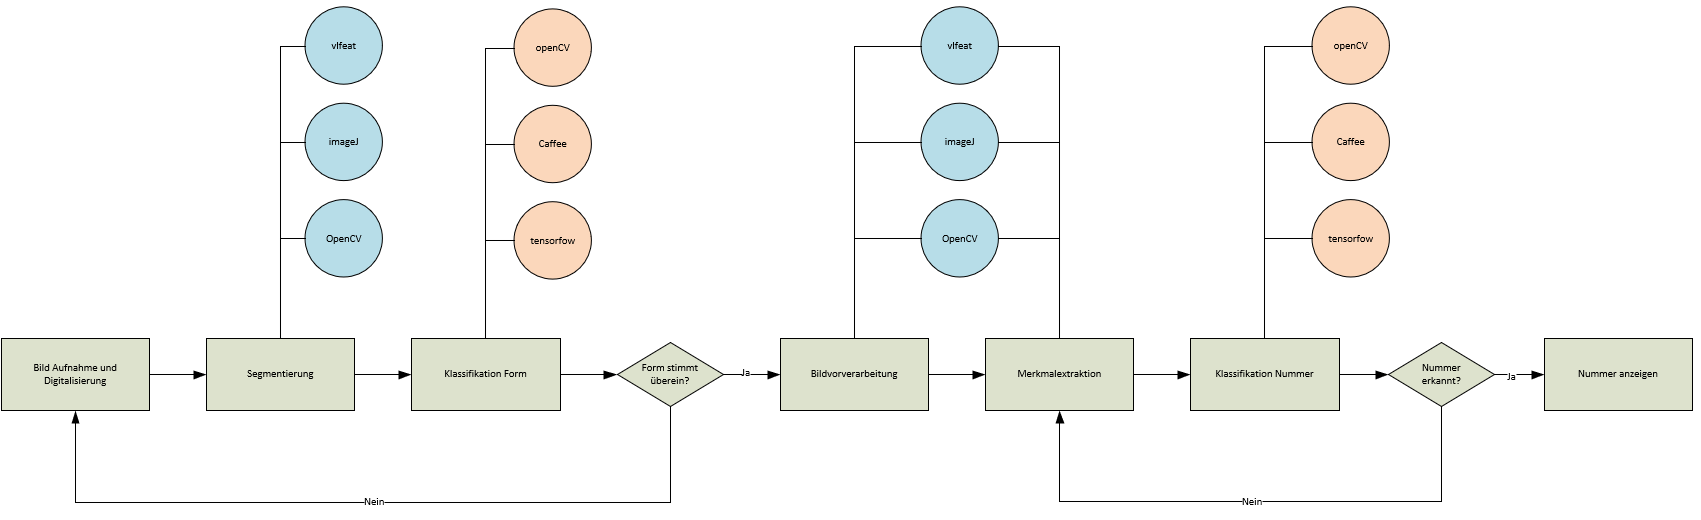
\includegraphics[width=1\textwidth]{Ablauf_vision.PNG}
    \end{figure}



\end{document}
